\documentclass[aspectratio=169]{beamer}
\usepackage[utf8]{inputenc}
\usepackage{bookman}
\usetheme{Dresden}
\usepackage{graphicx}
\usepackage{hyperref}

\title[02-EDA]{Introduction to Electronics Design Automation (EDA)\\Schematic Capture}
\author{MedTech Prototyping Skills (BME290L)}
\institute[Palmeri (Spring 2023)]{Mark L. Palmeri, M.D., Ph.D.}
\date{January 31, 2023}
\logo{
\includegraphics[width=0.1\textwidth]{BME-HorizontalLogo-Web-Blue.png}}

\begin{document}

\frame{\titlepage}

\frame{
    \frametitle{Outline}
    \tableofcontents
}

\section{Overview}

\frame{
    \begin{center}
        
\includegraphics[width=0.15\textwidth]{kicad_logo_small.png}
    \end{center}

    \begin{itemize}
        \item Installation: \url{https://kicad.org}
        \begin{itemize}
          \item Certain video cards will not work well with the PCB tool.  In that case, disable the \textit{Accelerated} toolset and choose the \textit{Fallback} graphics toolset.
          \item On Macs, your part / footprint / model libraries might not be detected automatically after installation.  You might need to manually point Kicad at them in a path similar to: \texttt{Macintosh/Library/Application Support/kicad/templates/sym-lib-table/}.
        \end{itemize}
        \item Documentation: \url{https://docs.kicad.org/6.0/en/getting_started_in_kicad/getting_started_in_kicad.html}
    \end{itemize}
}

\section{Schematics}

\frame{
  \frametitle{UI/UX}

  \centerline{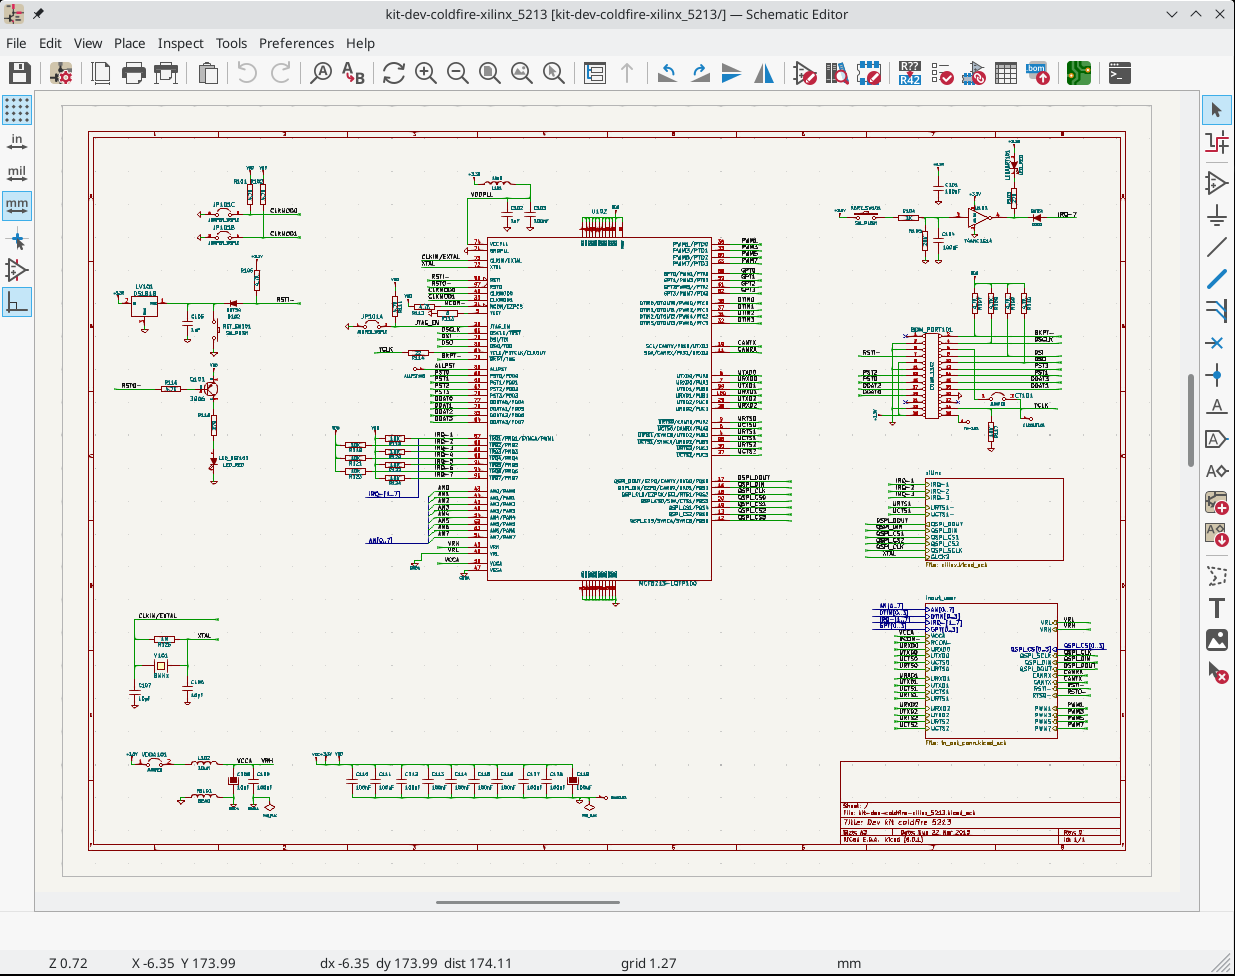
\includegraphics[width=0.5\textwidth]{commands_overview.png}}

  \begin{center}
    \begin{footnotesize}
      \url{https://docs.kicad.org/6.0/en/eeschema/eeschema.html\#schematic-editing-operations}
    \end{footnotesize}
  \end{center}
}

\frame{
  \frametitle{Schematic Capture}
  \begin{columns}
  \begin{column}{0.7\textwidth}
    \begin{enumerate}
      \item Create a New Project, which creates a schematic file.
      \item \textbf{DO NOT CHANGE THE GRID SPACING!!}
      \item Setup \texttt{Page Settings...}, using \href{https://semver.org/}{semantic versioning} for ``Revision''.
      \item Configure \texttt{Schematic Setup...}, including \texttt{Project:Net Classes}.
    \end{enumerate}
  \end{column}
  \begin{column}{0.3\textwidth}
    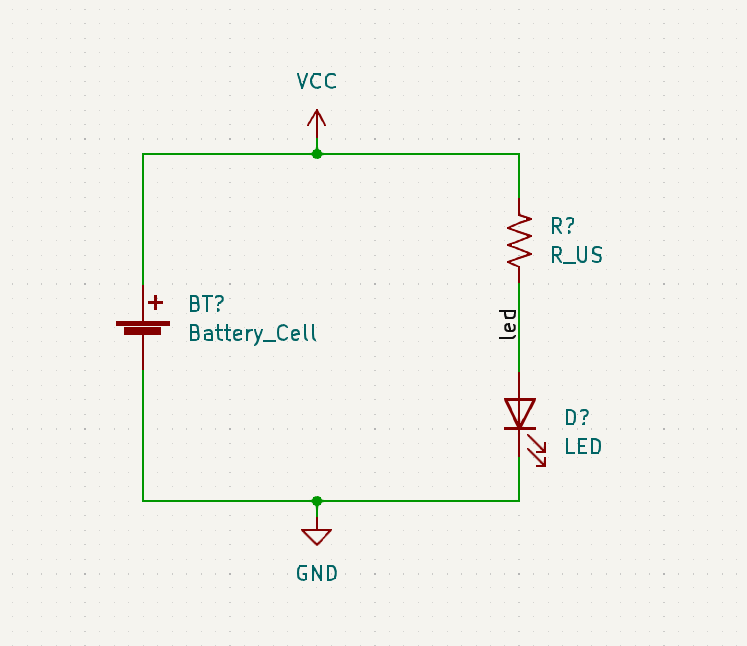
\includegraphics[width=1.0\textwidth]{symbols-labeled.png}
  \end{column}
  \end{columns}
}
	  
\begin{frame}
   \begin{columns}
    \begin{column}{0.6\textwidth}
      \begin{enumerate}
        \setcounter{enumi}{4}
        \item Place component / part (\texttt{Place Symbol}) using default library.
        If component doesn't exist, then you either need to:
        \begin{itemize}
          \item Download the part from an online database (e.g., \href{https://www.snapeda.com/}{SnapEDA})
          \item Create part using the \texttt{Library Editor}.
        \end{itemize}
        \item Annotate components (give each component a unique label)
        \item Assign component values
        \item Label nets with meaningful names
        \begin{itemize}
            \item Nets are like nodes; common voltage connections.
            \item Use Global net labels to avoid connection chaos.
        \end{itemize}
      \end{enumerate}
    \end{column}
    \begin{column}{0.4\textwidth}
      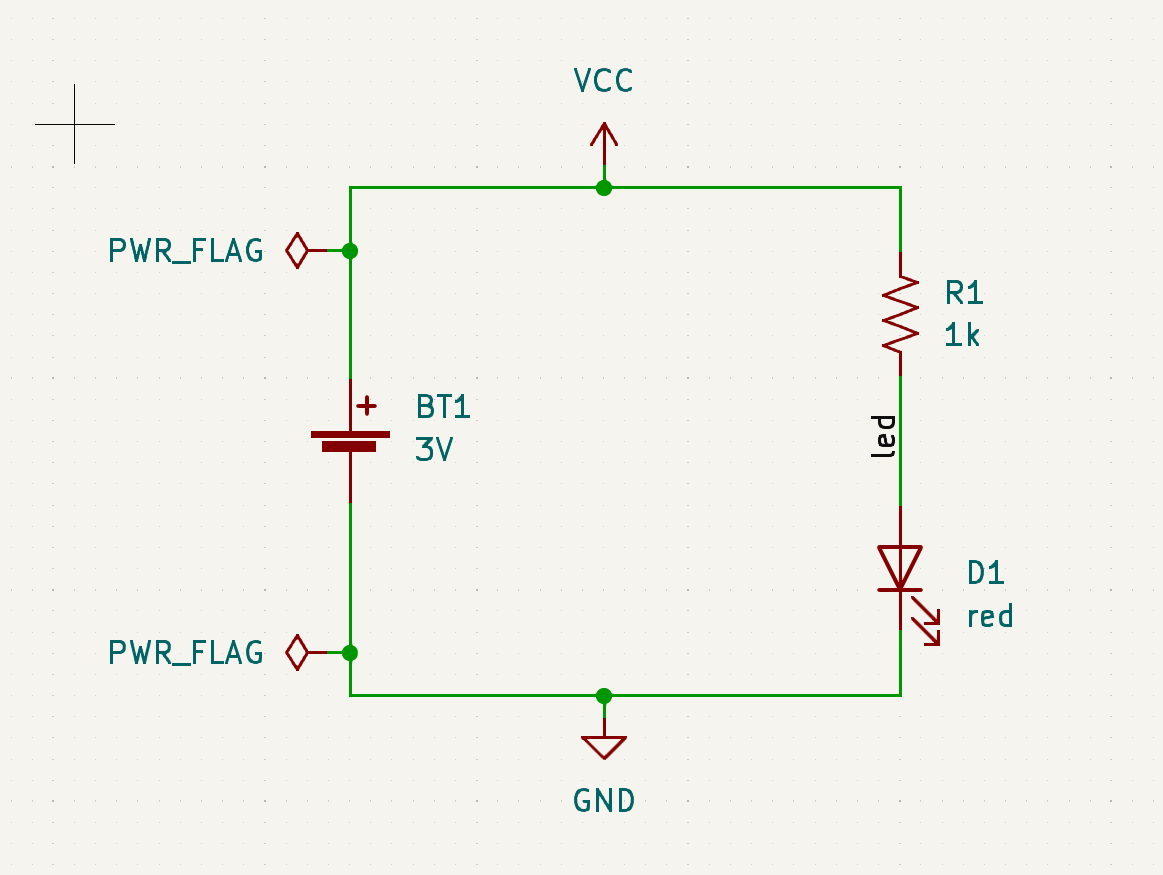
\includegraphics[width=1.0\textwidth]{symbols-pwr-flag.png}   
    \end{column}
   \end{columns}
\end{frame}

\section{Power}
\begin{frame}
  \frametitle{Power Ports}

  \begin{columns}
    \begin{column}{0.6\textwidth}
      \begin{itemize}
        \item Power ports, including ground references, are also global net labels.
        \item Component pins can be explicitly designated power in/out (in contrast to signal).
        \item Power, ideally, cascades top-to-bottom (\texttt{+} $\rightarrow$
        \texttt{GND} [$\rightarrow$ \texttt{-}]) on the schematic.
      \end{itemize}
    \end{column}
    \begin{column}{0.4\textwidth}
      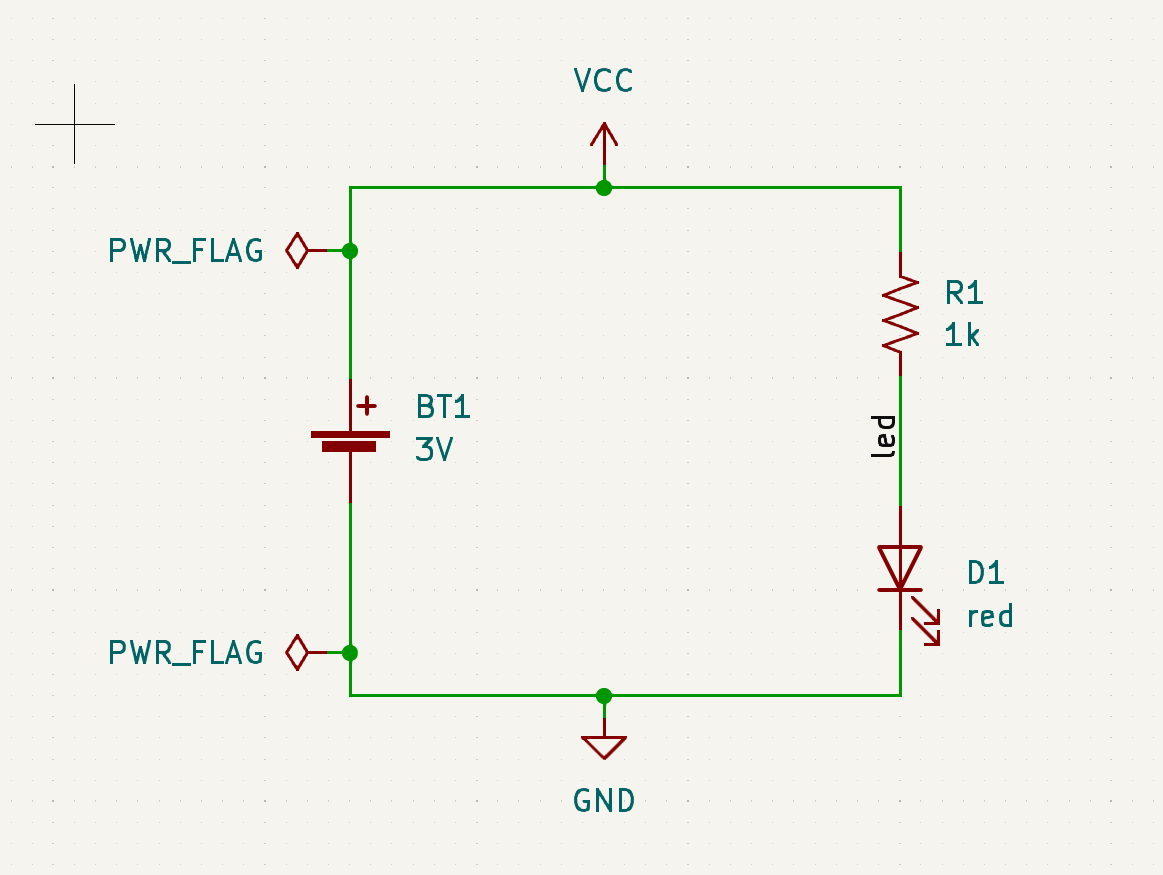
\includegraphics[width=1.0\textwidth]{symbols-pwr-flag.png}   
    \end{column}
\end{columns}
\end{frame}

\section{ERC}
\begin{frame}
  \frametitle{Electrical Rules Check (ERC)}
  \begin{columns}
    \begin{column}{0.6\textwidth}
      \begin{itemize}
        \item Check the validity of the schematic
        \item Common error: ``Input Power pin not driven by any Output Power pins''
        \begin{itemize}
          \item KiCad checks to make sure that power can ``drive'' components that demand that input.
          \item You can explicitly indicate this in the schematic using the
          \texttt{PWR\_FLAG} symbol attached to the net in question.
          \item Might need to re-map pin types (\texttt{Properties:Edit Symbol:Pin Table}).
        \end{itemize}
      \end{itemize}
    \end{column}
    \begin{column}{0.4\textwidth}
      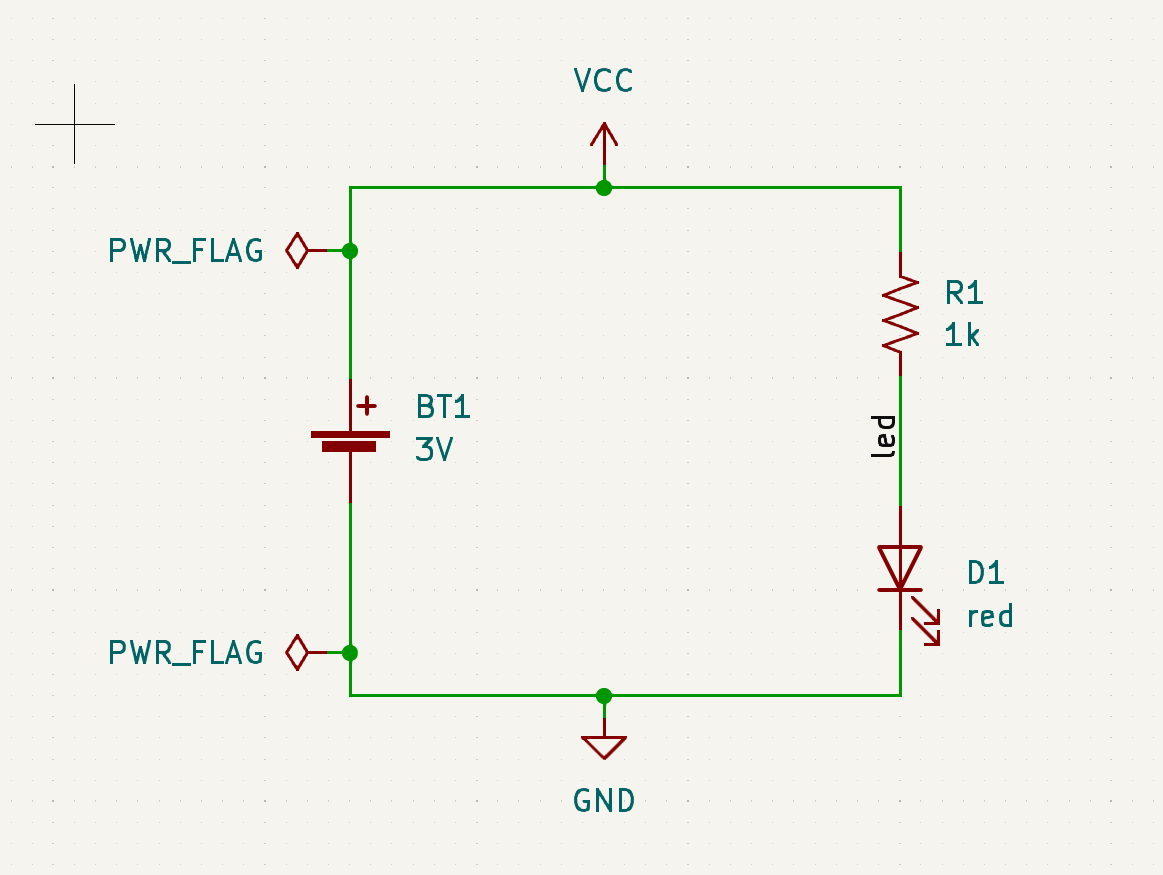
\includegraphics[width=1.0\textwidth]{symbols-pwr-flag.png}   
    \end{column}
  \end{columns}
\end{frame}

\section{Best Practices}
\frame{
   \frametitle{Best Practices}
   \begin{itemize}
      \item Signal, ideally, flows left-to-right (input $\rightarrow$ output).
      \item Outline and label functional blocks.  Use \texttt{Heirarchical
      Sheets} to organize more clearly-defined sub-circuits.
      \item Can include non-electrical items, like \texttt{Mounting Holes}.
      \item Add Test Pins/Pads to nets you will want to verify during testing.
      \begin{itemize}
        \item Power nets
        \item Signal I/O
      \end{itemize}
      \item Use \texttt{No-Connection} flags for pins that are intentionally
       not connected to other components.
      \item You can create a Bill of Materials (BOM) based on your schematic.
   \end{itemize}
 }

 \begin{frame}
  \centerline{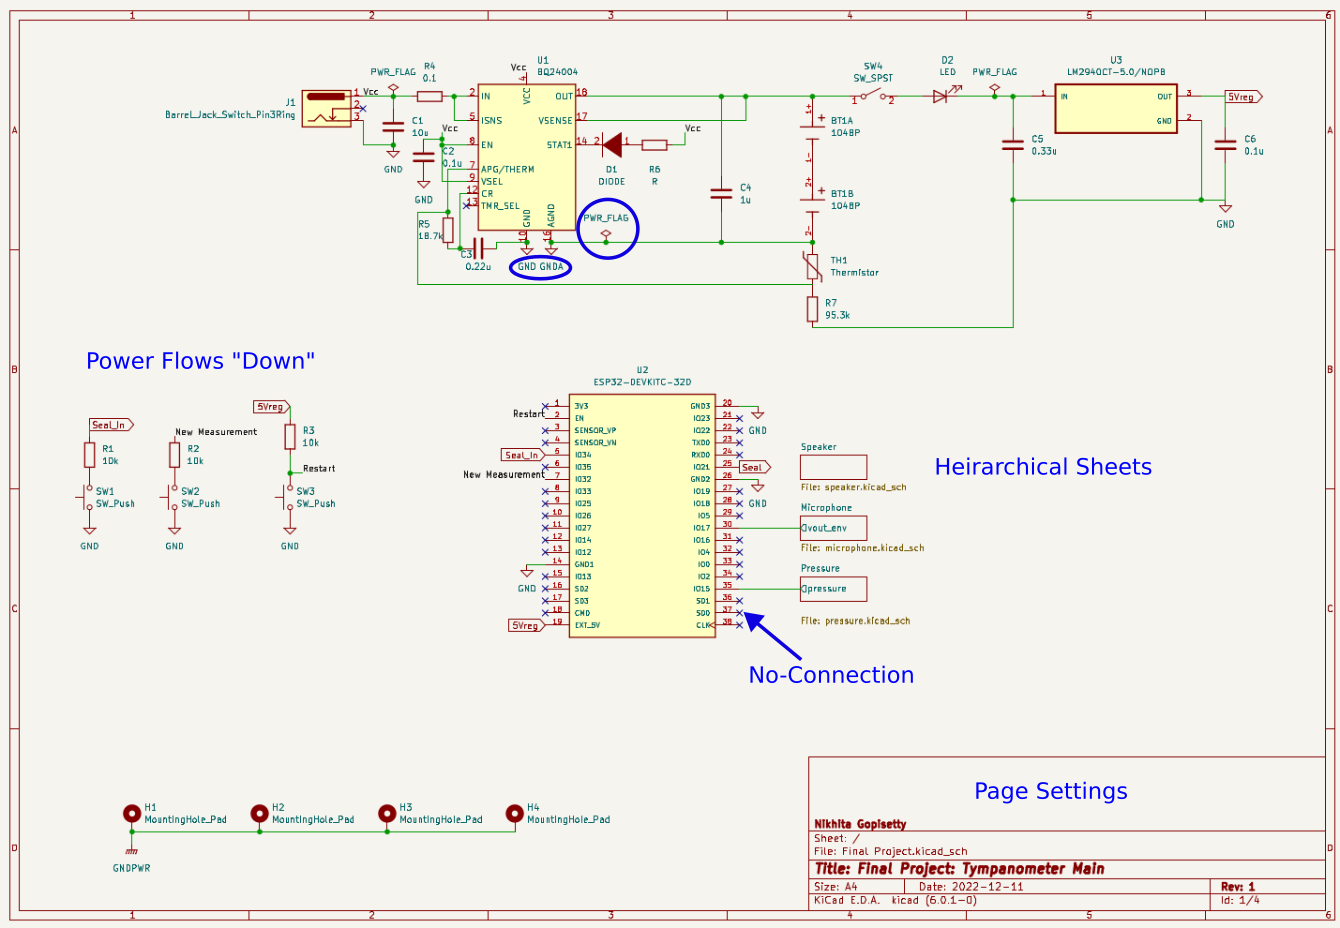
\includegraphics[width=0.7\textwidth]{schematic_annotated.png}}
 \end{frame}

\section{In-class Exercise}

\begin{frame}
  \frametitle{A current project...}

  \centerline{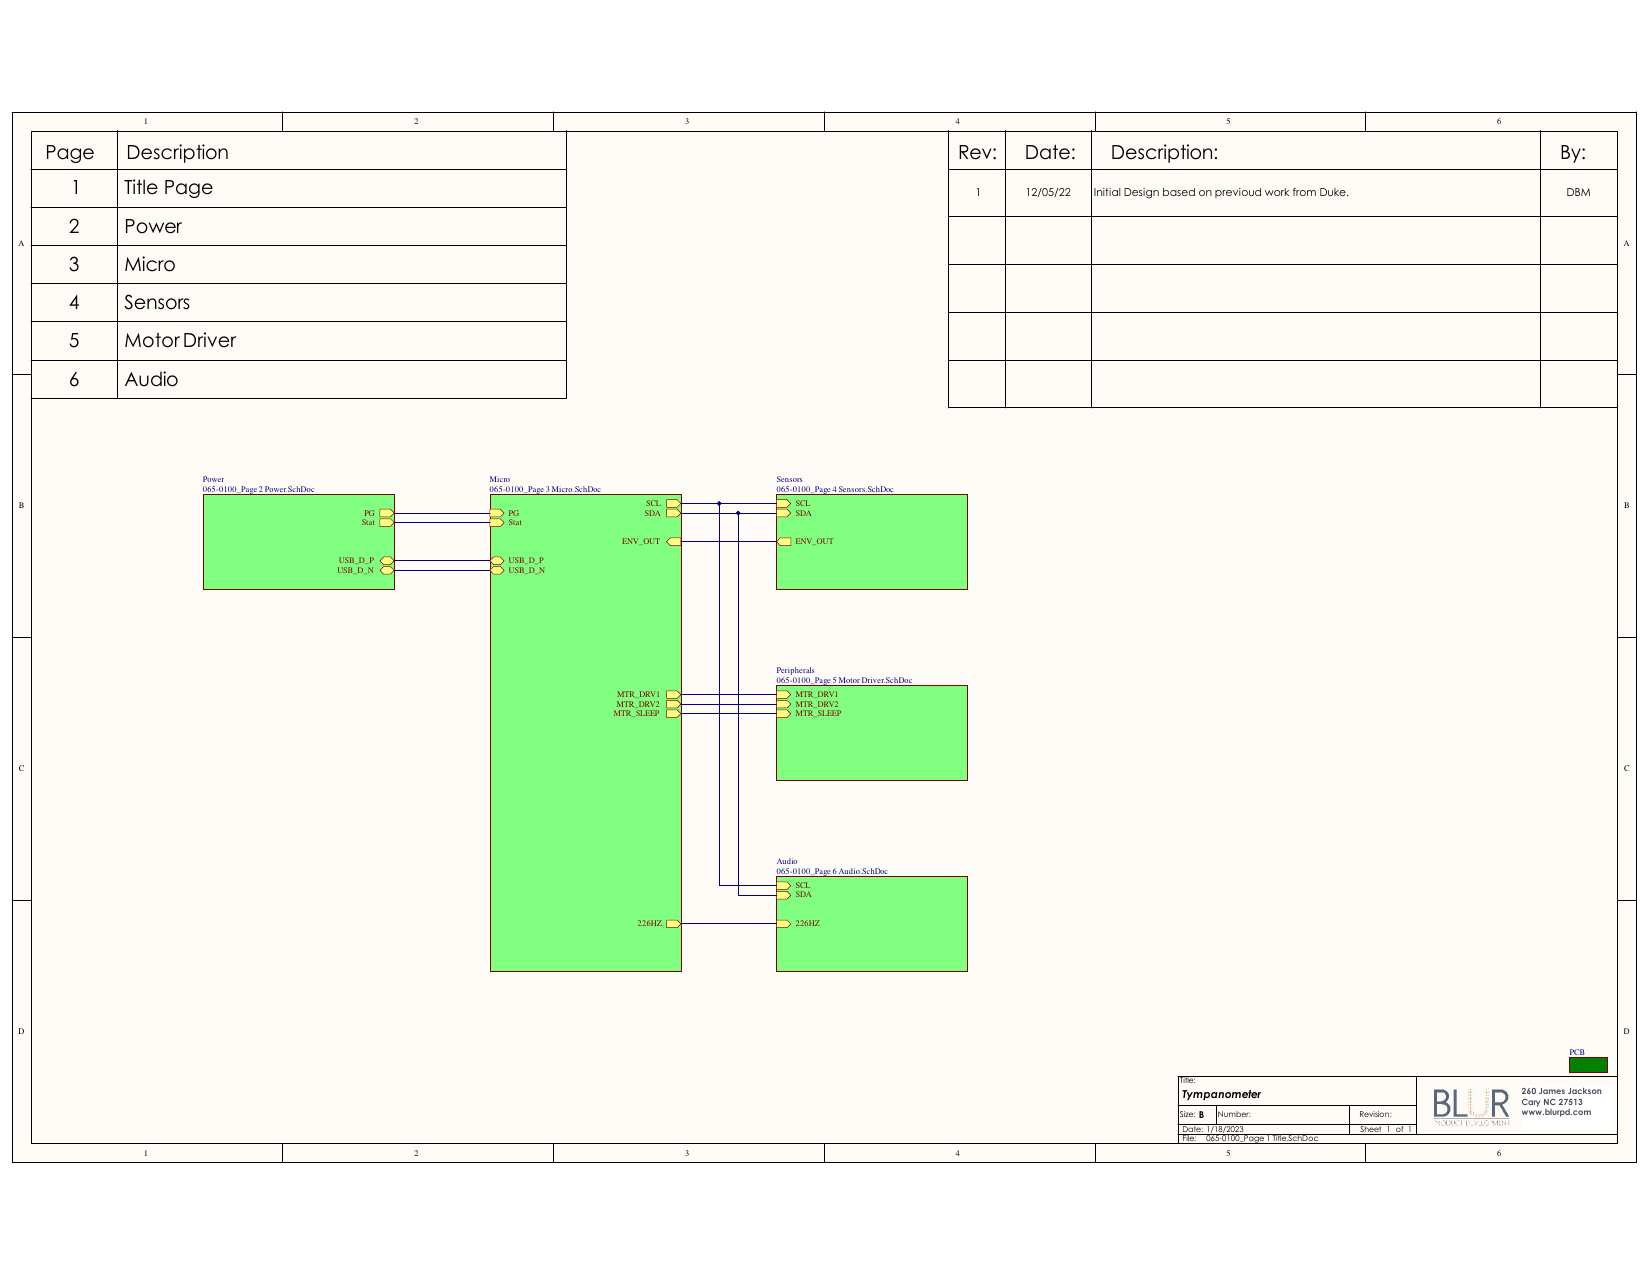
\includegraphics[width=0.6\textwidth]{065-0100_Main_Board-1.png}}
\end{frame}

\begin{frame}
  \frametitle{A current project...}

  \centerline{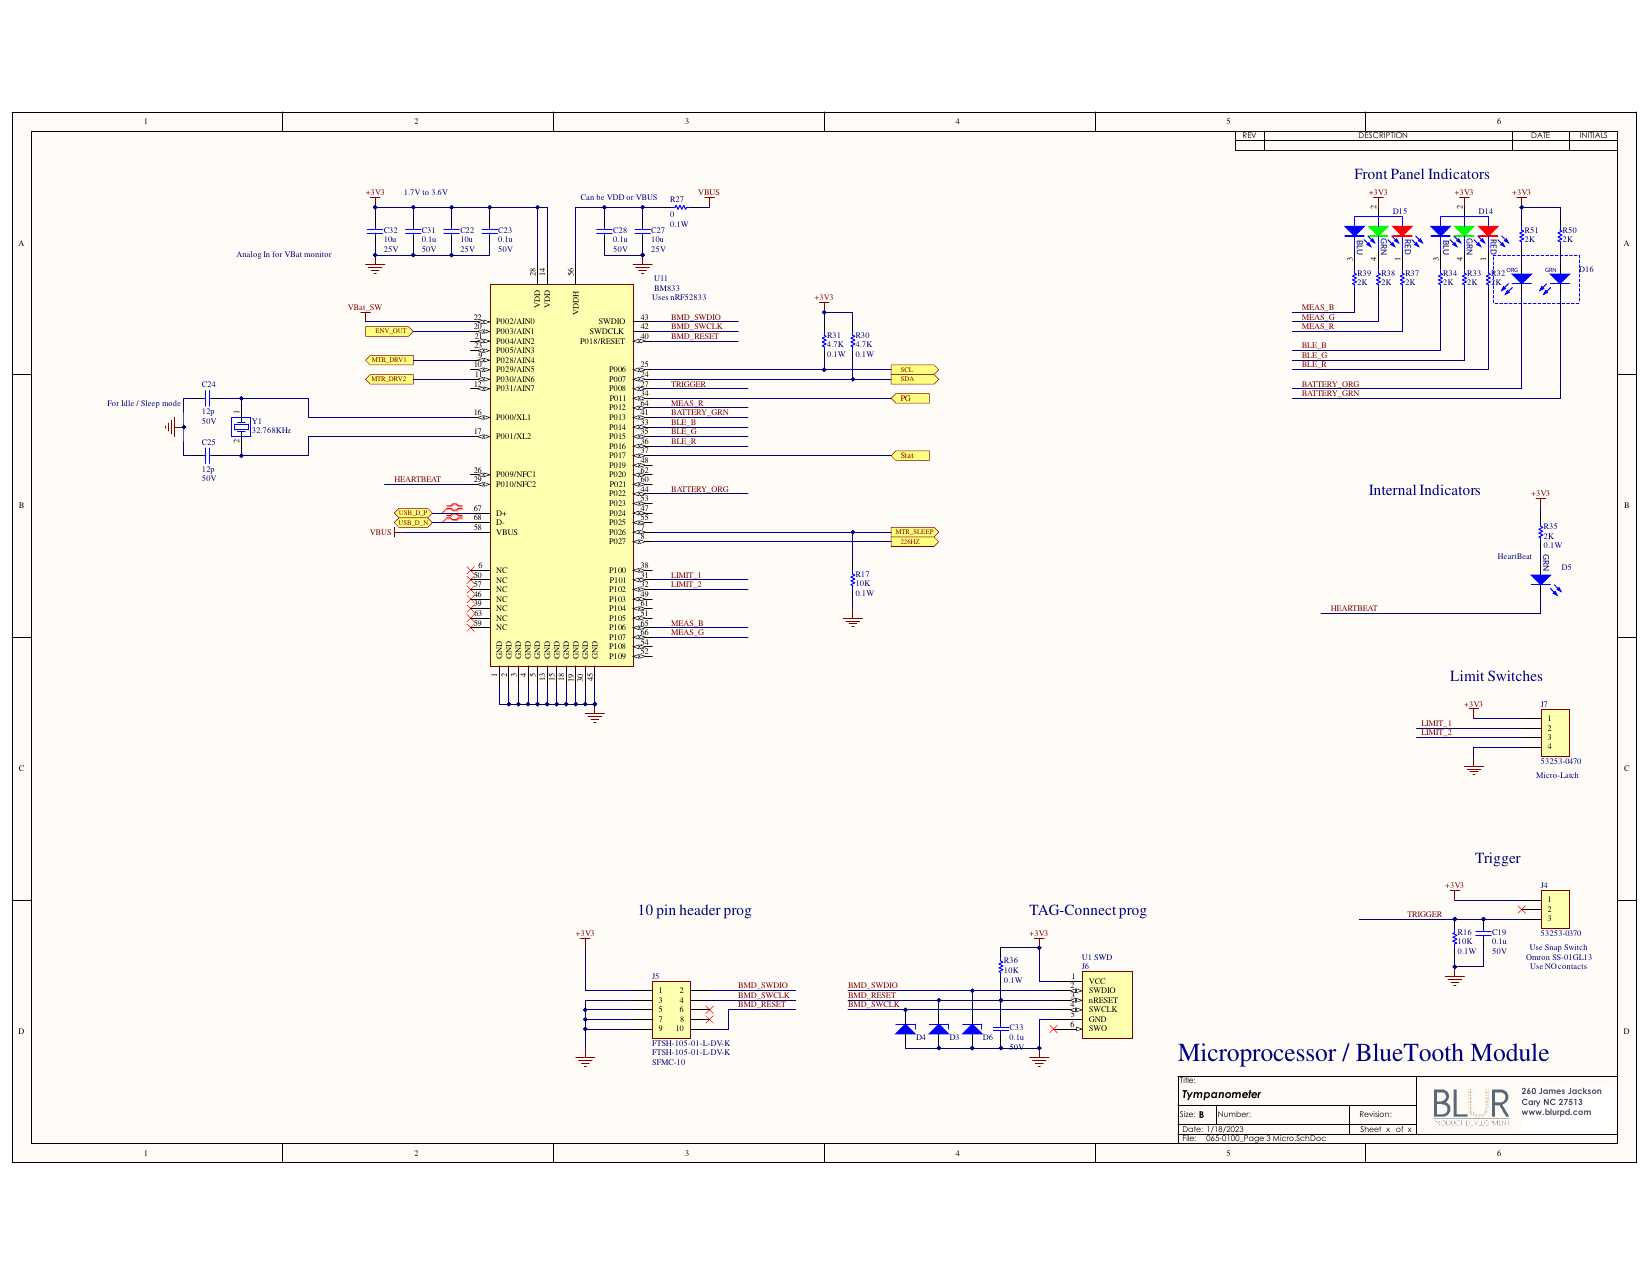
\includegraphics[width=0.6\textwidth]{065-0100_Main_Board-5.png}}
\end{frame}

\begin{frame}
  \frametitle{A current project...}

  \centerline{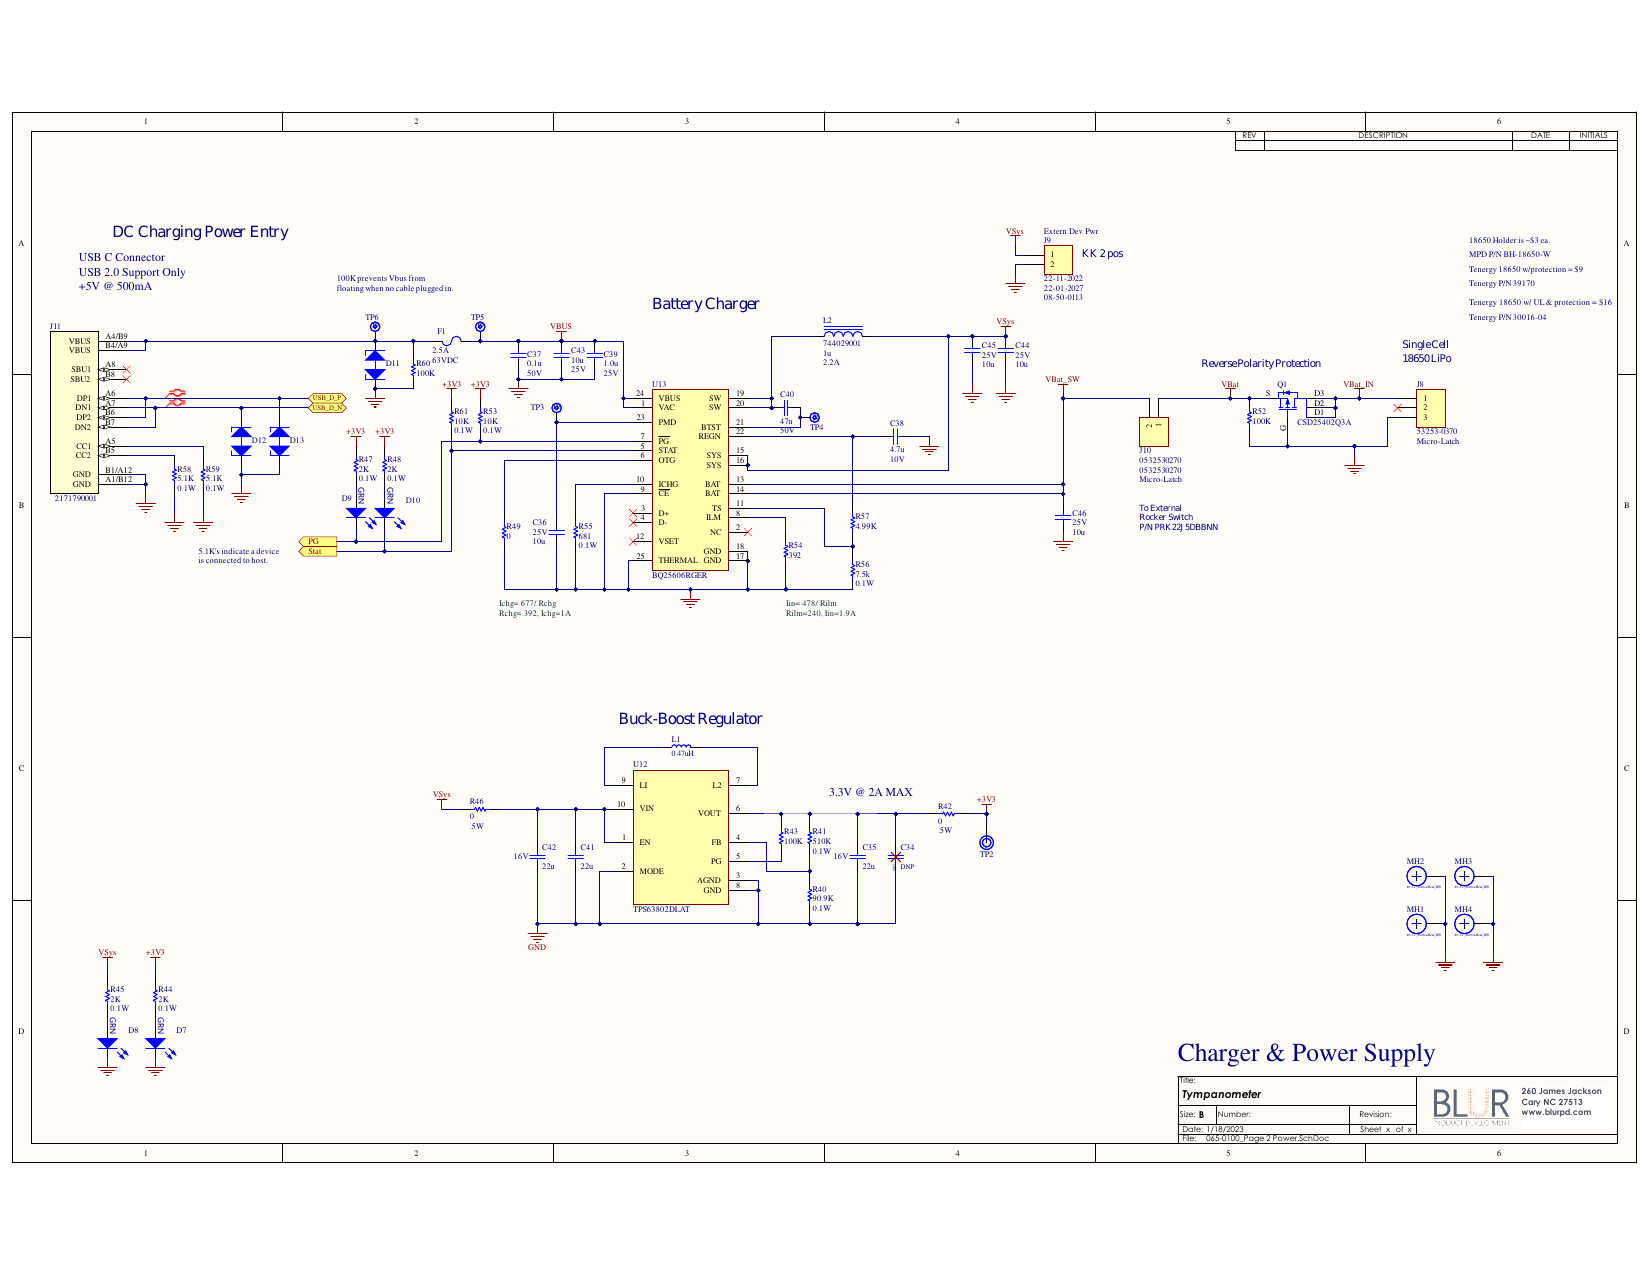
\includegraphics[width=0.6\textwidth]{065-0100_Main_Board-6.png}}
\end{frame}

\begin{frame}
  \frametitle{A current project...}

  \centerline{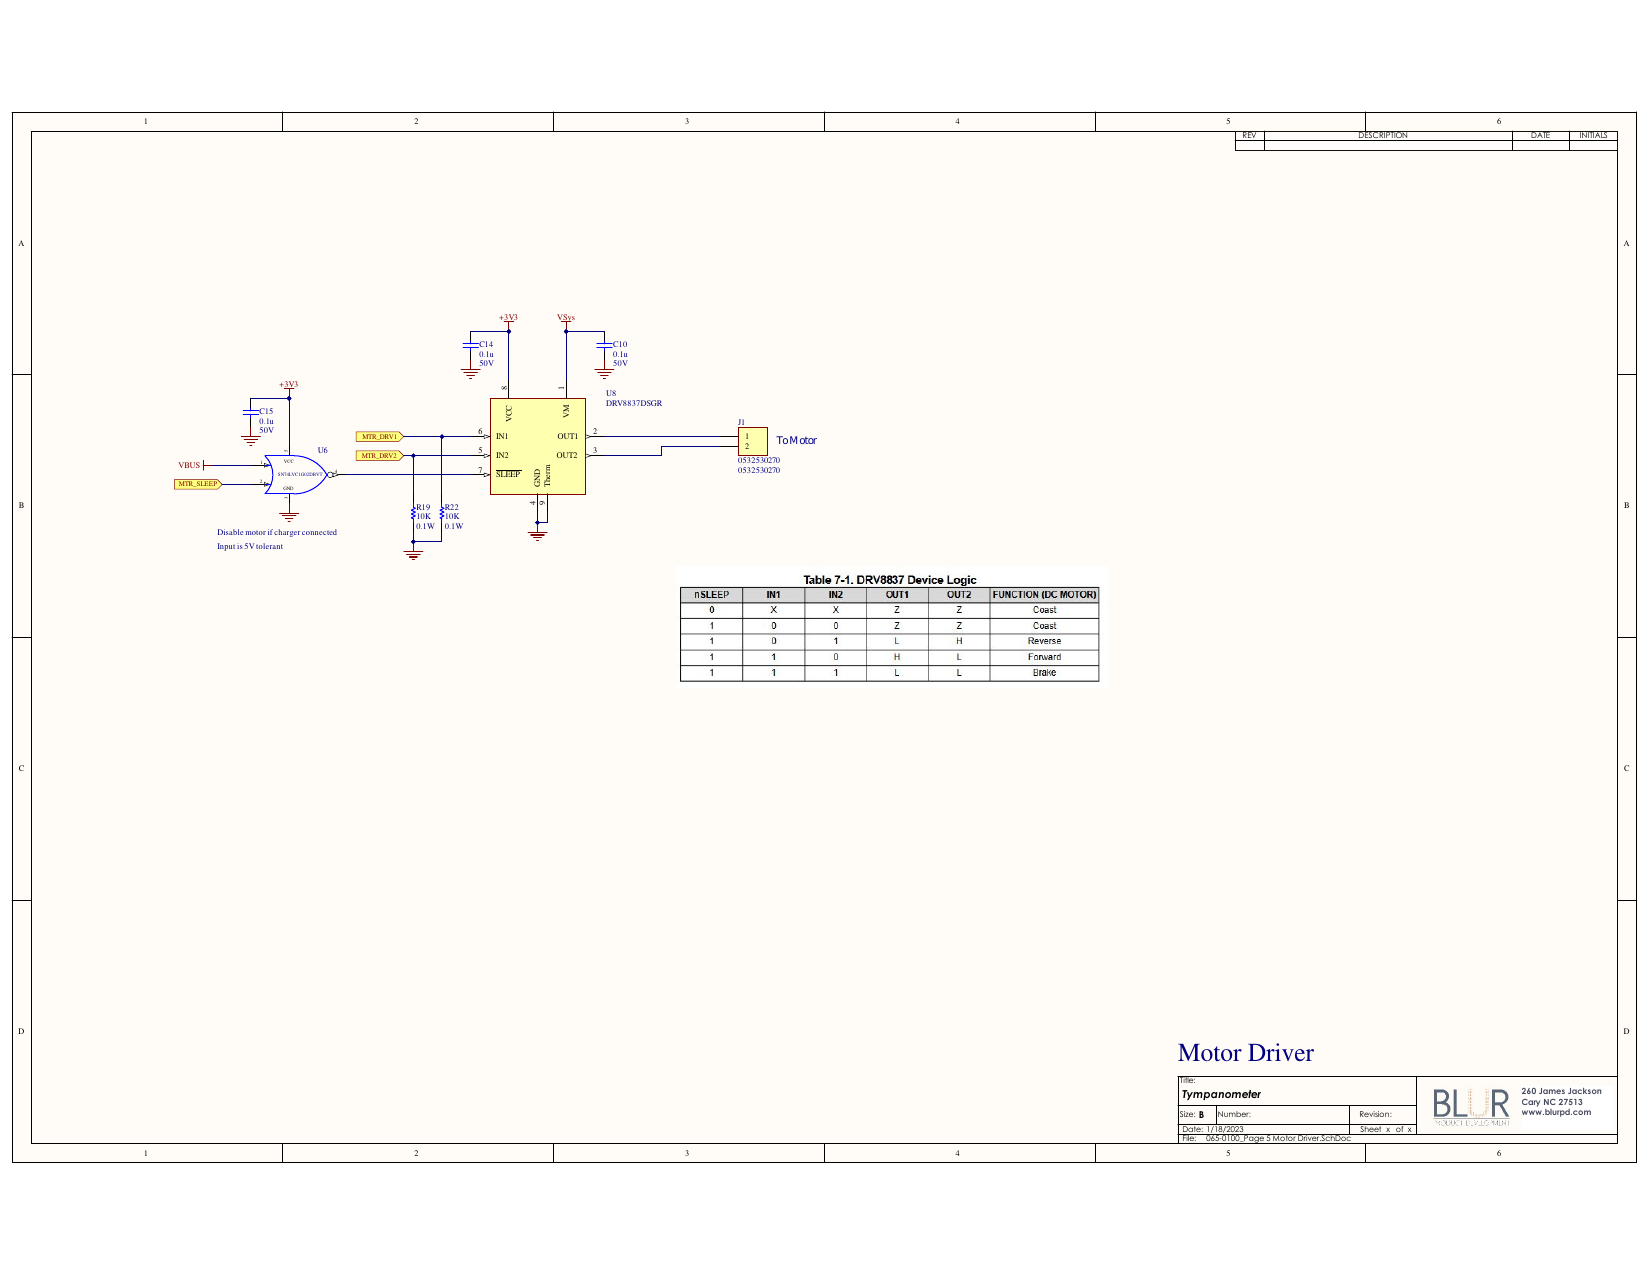
\includegraphics[width=0.6\textwidth]{065-0100_Main_Board-3.png}}
\end{frame}

\frame{
  \frametitle{Lets create the schematic for a battery voltage regulator...}
  \begin{itemize}
    \item \texttt{File $\rightarrow$ Page Settings$\dots$}
    \item \texttt{File $\rightarrow$ Schematic Setup$\dots$} (add Power net class)
    \item 4 AA battery
    \item \texttt{7805} voltage regulator
    \item Use power ports for battery voltage and \texttt{GND}.
    \item Annotate components
    \item Test pin on each net
    \item Label \texttt{Vout} net.
    \item Create a \texttt{Heirarchical Sheet} for a load.
  \end{itemize}

}

\begin{frame}
  \frametitle{In lab this week...}

  More schematic generation fun!
\end{frame}

\end{document}
